\documentclass[journal]{IEEEtran}

\usepackage{cite}
\usepackage{texnames}
\usepackage{graphicx}
\graphicspath{{}{}}
\DeclareGraphicsExtensions{.pdf,.jpeg,.png}

\usepackage{amsmath}
\interdisplaylinepenalty=2500
\usepackage{algorithmic}
\usepackage{array}
\usepackage[caption=false,font=footnotesize]{subfig}
\usepackage{dblfloatfix}
%\usepackage[nomarkers]{endfloat}
\usepackage{url}
\usepackage{booktabs}

\usepackage{tikz}
\usetikzlibrary{shapes.geometric,arrows,trees}


\tikzstyle{root} = [rectangle, rounded corners, minimum width=2cm, minimum height=.7cm, text centered, draw=black, fill=blue!30]
\tikzstyle{files} = [rectangle, minimum width=1cm, minimum height=.5cm, text centered, draw=black, fill=white]
\tikzstyle{link} = [thick, -]

\begin{document}
	
\title{Grading Reproducibility in Remote Sensing Articles}
	
\author{Alejandro~C.~Frery,~\IEEEmembership{Senior Member,~IEEE,}
Luis~Gomez,~\IEEEmembership{Senior Member,~IEEE,}
and~Qi~Wang,~\IEEEmembership{Senior Member,~IEEE}% <-this % stops a space
\thanks{A.\ C.\ Frery is with the \textit{Laborat\'orio de Computa\c c\~ao Cient\'ifica e An\'alise Num\'erica} -- LaCCAN, Universidade Federal de Alagoas, Macei\'o, Brazil (email: acfrery@laccan.ufal.br)}% <-this % stops a space
\thanks{Luis Gomez is with the Universidad de Las Palmas de Gran Canaria, Spain}% <-this % stops a space
\thanks{Qi Wang is with the Northwestern Polytechnical University, China}% <-this % stops a space
\thanks{Manuscript received XX, accepted YY.}}
	
\markboth{IEEE Journal of Selected Topics on Applied Earth Observations and Remote Sensing,~Vol.~XX, No.~YY, Month~2020}%
{Frery \MakeLowercase{\textit{et al.}}: Grading Reproducibility}
	
\maketitle
	
\begin{abstract}
The abstract goes here.
\end{abstract}
	
\begin{IEEEkeywords}
Reproducibility,
Replicability,
Remote Sensing
\end{IEEEkeywords}
	

\IEEEpeerreviewmaketitle

\section{Introduction}
	
\IEEEPARstart{R}{eproducibility} is at the core of experimental sciences. 
It is also a basilar element of scientific integrity. 
The advent of data science is leading to new requirements and practices able to cope with the challenges posed by huge volumes of data, often of dynamic nature. 
	
Modern grounds for Reproducible Research were set before the widespread use of deep learning and other massively data-based techniques. 
	
Among the efforts made towards building Remote Sensing Reproducible Research environments, one may mention Code Ocean and GRSS Remote Sensing Code Library. 
These two initiatives belong to the IEEE scientific ecosystem. 
	
However, is this enough for healthy science in Remote Sensing? 
We do not think so. 
Many authors continuously strive to disseminate their research findings in such a way that any user will be able to validate them at a later stage. 
This includes the proposal of software architectures, the use of open data, FLOSS (Free/Libre Open Source Software), and other initiatives.
		
Universally accessible and informative web page containing:
	\begin{enumerate}
		\item\label{item:ProjectID} Project identification (one project may host more than one paper; one paper may be hosted by more than one project)
		\begin{enumerate}
			\item Title
			\item Participants
			\item Summary
			\item Funding information
			\item Start date, state (in preparation, active, finished)
		\end{enumerate}
		\item Paper identification (if different from~\ref{item:ProjectID})
		\begin{enumerate}
			\item Title
			\item Authors (all authors with contact: at least, email and institution) with their institutions (at least one institution with address: that of the corresponding author)
			\item Abstract
			\item PDFs of relevant versions, including information of its submission to repositories (arXiv, etc.), journal or conference
			\item\label{item:SourceDocumentFiles} \LaTeX\ and \BibTeX\ files, images, and plots
		\end{enumerate}
		\item Computational platform (machine, model, operating system, software, libraries, and versions)
		\item Code (with comments)
		\item Data
		\item Which software components are FLOSS or free (including operating system)?
		\item How to install and run the code (instructions and examples)
		\item How to read and modify the data \item How to generate the plots, images (where they improved for visualization? how?), and tables (rounding, truncating, etc.)
		
	\end{enumerate}
	
	
	\begin{table*}[hbt]
		\centering
		\caption{Reproducibility scores of a research paper for the Remote Sensing community}
		\label{tab:my_label}
		\begin{tabular}{rccc}\toprule
			Question    & Answer & Score \\ \midrule
			1           & Does the project have a universally accessible web page & Yes & \\ 
			&  \\
			& \\ \bottomrule
		\end{tabular}
	\end{table*}

\section{How to Start Writing a Reproducible Article}

Starting well saves lots of time.
Here we make simple recommendations that may save time and efforts.
We assume that you use \LaTeX\ and \BibTeX.

The main idea consists in having a single repository for all the scientific texts you write: 
theses, 
reports, 
articles, 
letters,
reviews,
and miscellaneous documents.

Fig.~\ref{Fig:StructRepo} illustrates the recommended basic structure for a repository holding several \LaTeX\ files (or projects), along with their associated data and code.

Every directory may contain specific subdirectories.
For instance, \verb|Data| may contain \verb|CSV|, \verb|text|, and other directories with specific data files.

Notice that there is a single \BibTeX\ file (with extension \verb|.bib| in the \verb|Common| directory).
\BibTeX\ references can be split on several files, but these files should be common to all projects.
This avoids outdated and redundant bibliographic data bases.

Every article should be in its pwn directory.
Avoid using the name of the journal where you will submit your work for the directory and document names, as the destination may change along the process.

Data, figures, images and code should be common to all projects, as one typically reuses them.

Check Ref.~\cite{EditorialGRSL2015} for naming convention and revision handling of submitted manuscripts.

\begin{figure}[hbt]
\centering
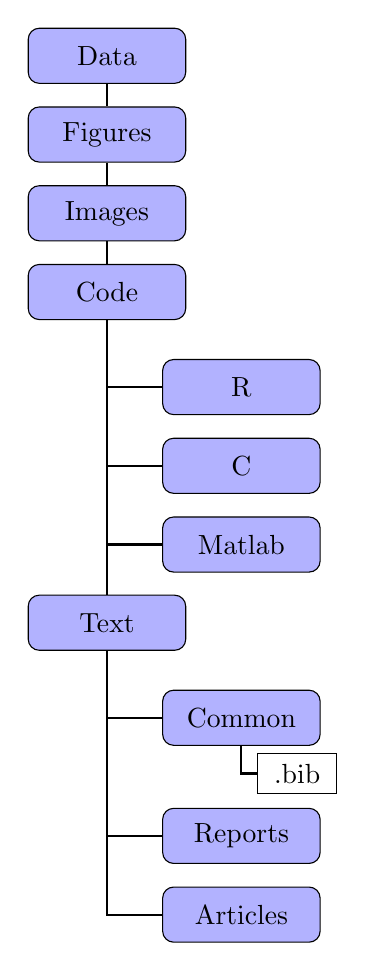
\begin{tikzpicture}[node distance=1cm,scale=.5]

\node (data) [root] {Data};
\node (figures) [root, below of=data] {Figures};
\node (images) [root, below of=figures] {Images};
%
\node (code) [root, below of=images] {Code};
	\node (R) [root, below right of=code, xshift=1cm, yshift=-.5cm] {R};
	\node (C) [root, below of=R] {C};
	\node (Matlab) [root, below of=C] {Matlab};
%
\node (text) [root, below of=code, yshift=-3.2cm] {Text};
	\node (common) [root, below right of=text, xshift=1cm, yshift=-.5cm] {Common};
	\node (biblio) [files, below right of=common] {.bib};
	\node (reports) [root, below of=common, yshift=-.5cm] {Reports};
	\node (articles) [root, below of=reports] {Articles};
%
\draw [link] (data) -- (figures);
\draw [link] (figures) -- (images);
\draw [link] (images) -- (code);
	\draw [link] (code) |- (R);
	\draw [link] (code) |- (C);
	\draw [link] (code) |- (Matlab);
\draw [link] (code) -- (text);
	\draw [link] (text) |- (common);
		\draw [link] (common) |- (biblio);
	\draw [link] (text) |- (reports);
	\draw [link] (text) |- (articles);
\end{tikzpicture}
\caption{Recommended structure of a repository for scientific texts}\label{Fig:StructRepo}
\end{figure}
	
\section{Conclusion}
The conclusion goes here.
	
\section*{Acknowledgments}
The authors would like to thank...
	
\nocite{StatisticalAnalysesReproducibleResearch,%
RRComputationalHarmonicAnalysis,%
RREconometrics,%
RRSignalProcessing,%
AddressingNeedDataCodeSharingComputationalScience,%
ReproducibleResearchinComputationalScience,%
TenRulesReproducibleComputationalResearch,%
ManifestoReproducibleScience}
	
\bibliographystyle{IEEEtran}
\bibliography{../Common/references}
	
%\begin{IEEEbiography}[{\includegraphics[width=1in,height=1.25in,clip,keepaspectratio]{mshell}}]{Michael Shell}
%% or if you just want to reserve a space for a photo:
%\end{IEEEbiography}
	
\end{document}


